\documentclass[11pt,a4paper]{article}
\usepackage[ngerman]{babel}
\usepackage{fontspec,amsmath,amssymb,graphicx,geometry,booktabs,longtable,array,float,hyperref}
\geometry{margin=25mm}
\setmainfont{Latin Modern Roman}
\hypersetup{colorlinks=true,linkcolor=blue,urlcolor=blue}
\emergencystretch=3em
\sloppy
\setcounter{secnumdepth}{0}
\setlength{\parindent}{0pt}
\setlength{\parskip}{0.5em}
\begin{document}
\tableofcontents
\newpage

\section*{FEM-Ersatzmodelle für einen parametrischen Balken}
\section{Wissenschaftlich-technische Ausarbeitung des bisherigen Projektstands}
Stand: 26. Oktober 2026. Diese Ausarbeitung rekonstruiert vorhandene Berechnungen; für ihre Erstellung wurden keine FEM-Läufe oder Modelltrainings gestartet. Historische Berichte und Primärdateien werden im Text unterschieden.

\subsection{Kurzfassung}
Das Projekt untersucht, wie sich Verschiebungsfelder und Eigenfrequenzen eines parametrischen, einseitig eingespannten Balkens aus wenigen Finite-Elemente-Berechnungen (FEM) annähern lassen. Solche Ersatzmodelle können wiederholte Berechnungen beschleunigen. Die bisherige Geometrie ist ein Quader, kein Elektromotor; eine Übertragung auf einen Motor ist eine zukünftige Forschungsfrage.

In der historischen statischen Reihe sank der Medianfehler des direkten POD-GPR bei 12 bis 384 Trainingsfällen auf den sechs mehrfach betrachteten Testfällen von 60,652 \% auf 0,384 \%. Die Verfahren liefern unterschiedliche Ausgaben und besitzen unterschiedliche Onlinekosten. Die Zahl sechs bezeichnet sechs Parameterkombinationen, nicht 525 räumliche Punkte oder sechs Moden pro Fall.

In einem späteren Vergleich mit 18 Trainingsfällen war die analytische Balkennäherung bereits stark: ihr mittlerer Feldfehler auf sechs internen Validierungsfällen lag bei 0,5215 \%. Die eingefrorene Hybridvariante lag bei 0,8544 \%, das direkte POD-GPR bei 113,834 \%. Eine später untersuchte Last-/Steifigkeitsnormierung reduzierte die Mittelwerte auf 0,1289 \% beziehungsweise 10,687 \%. Dies sind Entwicklungsbefunde, keine unabhängige Bestätigung.

Für die Modalanalyse wurden zwölf Trainings-, sechs Validierungs- und sechs Testfälle berechnet. Ein Frequenz-GPR erreichte auf den sechs historischen Testfällen über die ersten sechs Frequenzen einen mittleren relativen Fehler von 3,366 \%. Es prognostiziert das sortierte Frequenzspektrum; eigenständige Eigenform-Surrogate und modale Hybridmodelle sind nicht implementiert. Die erfassten Netz- und Dichteprüfungen betreffen wenige Konfigurationen.

\section{1. Ziel, Aufgaben und Forschungsfragen}
Ein FEM-Modell bildet Gleichgewicht und Materialgesetz räumlich auf einem Netz ab. Für eine Parameterstudie muss die Gleichung für viele Geometrien und Materialwerte erneut gelöst werden. Ein Ersatzmodell verschiebt einen Teil dieser Arbeit in eine Offlinephase: Zunächst werden Referenzlösungen erzeugt und ein Modell aufgebaut. Online wird für neue Parameter eine Vorhersage berechnet. Der Nutzen entsteht nur, wenn der Aufbauaufwand und die Genauigkeit zum späteren Einsatzzweck passen.

Die Studie vergleicht drei grundsätzlich verschiedene Ausgaben. Eine statische Verschiebung beschreibt die Verformung unter einer vorgegebenen Last. Eine Eigenfrequenz ist eine Kennzahl des freien linearen Schwingungsproblems. Eine Eigenform beschreibt die räumliche Form einer freien Schwingung. Die letzte ist vorzeichen- und skalierungsmehrdeutig. Ein Modell, das sechs Zahlen vorhersagt, löst daher nicht automatisch dieselbe Aufgabe wie eines, das ein Verschiebungsfeld oder Eigenformen liefert.

Im Zentrum stehen drei Fragen: Wie viele unabhängige Parameterfälle benötigt ein Verfahren? Welche Fehler bleiben auf nicht zum Training verwendeten Fällen? Welche Rechenoperationen fallen online tatsächlich an? Ein reduziertes Ordnungsmodell (ROM) mit erneuter Matrixassemblierung kann eine gute Genauigkeit erreichen, ohne dieselben Kosten wie ein rein datengetriebenes Modell zu haben.

\section{2. Referenzproblem und Parameter}
Der Körper ist ein Quader der Länge $L$, Breite $b$ und Höhe $h$. Das Koordinatensystem hat den Mittelpunkt der Länge und Breite bei null: $x\in[-L/2,L/2]$, $y\in[-b/2,b/2]$ und $z\in[0,h]$. Die Fläche bei $x=-L/2$ ist vollständig eingespannt. Auf der freien Fläche wirkt die gleichmäßig verteilte Kraftdichte $(0,0,F_z/(bh))$ in Pascal. Die Resultierende ist $F_z$; negative Werte wirken in negativer $z$-Richtung.

\begingroup\small\begin{longtable}{>{\raggedright\arraybackslash}p{0.200\textwidth}>{\raggedright\arraybackslash}p{0.200\textwidth}>{\raggedright\arraybackslash}p{0.200\textwidth}>{\raggedright\arraybackslash}p{0.200\textwidth}}
\toprule
Größe & Bereich & Einheit & Bedeutung\\ \midrule\endhead
$L$ & 0,6 bis 1,2 & m & Balkenlänge\\
$b$ & 0,06 bis 0,10 & m & Breite\\
$h$ & 0,08 bis 0,14 & m & Höhe\\
$E$ & 70 bis 210 & GPa & Elastizitätsmodul\\
$\nu$ & 0,25 bis 0,35 & 1 & Querkontraktionszahl\\
$F_z$ & −1000 bis −100 & N & gesamte statische Stirnlast\\
$\rho$ & 7850 & kg/m³ & konstante Demonstrationsdichte der Modalstudie\\
\bottomrule\end{longtable}\endgroup
Quelle: Projektkonfiguration config.m; die Dichte folgt dem Modal-Integrationsskript. Der Bereich ist ein Demonstrationsraum, keine Materialkalibrierung. Das Material ist homogen, isotrop und linear elastisch. Kleine Verformungen werden angenommen; die statische Routine enthält einen Grenzwert von 0,02 für das Verhältnis aus beobachteter Gitterverschiebung und Länge.

Für kleine Dehnungen beschreibt das isotrope Hooke-Gesetz den Zusammenhang zwischen Dehnung $\varepsilon$ und Spannung $\sigma_{\rm mech}$:

\[\sigma_{\rm mech}=\lambda\,\operatorname{tr}(\varepsilon)I+2G\varepsilon,\qquad G={E\over2(1+\nu)},\quad \lambda={E\nu\over(1+\nu)(1-2\nu)}.\]
Die Lamé-Konstanten $G$ und $\lambda$ besitzen die Einheit Pascal. Die mechanische Spannung $\sigma_{\rm mech}$ ist nicht mit dem später verwendeten GPR-Rauschparameter $\sigma$ zu verwechseln.

\[K(\mu)u(\mu)=f(\mu).\]
Hier sind $\mu=(L,b,h,E,\nu,F_z)$ die Parameter, $K$ die Steifigkeitsmatrix, $u$ die nodalen Verschiebungen in Metern und $f$ der Lastvektor in Newton. Die Einspannung wird als feste Randbedingung gesetzt. Die Implementierung src/solve\_\allowbreak{}case.m verwendet MATLABs femodel mit structuralStatic, generateMesh und solve; der Standard ist ein quadratisches Tetraedernetz mit $H_{\max}=\min(b,h)/3$. MATLAB wählt solverinterne Details; separat protokollierte iterative Solver oder Toleranzen sind den vorhandenen Aufzeichnungen nicht zu entnehmen.

Die freie, ungedämpfte und nicht vorgespannte Modalrechnung löst dagegen

\[K(\mu)\phi_i=\omega_i^2M(\mu)\phi_i,\qquad f_i=\omega_i/(2\pi).\]
$M$ ist die Massenmatrix, $\omega_i$ die Kreisfrequenz in rad/s und $f_i$ die Frequenz in Hz. Die statische Last ist kein Eingang des Modalproblems. Eine Eigenform $\phi_i$ kann mit beliebigem nichtnulligem Faktor multipliziert werden, ohne die Eigenwertgleichung zu ändern. Ihre Normierung legt deshalb keine Betriebsamplitude fest. Für eine zeitabhängige Betriebsschwingung wären Anregung, Anfangsbedingungen und gegebenenfalls Dämpfung nötig.

Das Modalbackend +femstudy/+fem/modal.m nutzt structuralModal, quadratische Elemente und dieselbe Einspannung. Das Frequenzsuchintervall beginnt bei 2000 Hz und wird bei Bedarf verdoppelt, bis mindestens acht Moden verfügbar sind; davon sind sechs Ziele und weitere Moden Puffer für die Zuordnung. Die gespeicherten Obergrenzen und Netzgrößen stehen in den einzelnen Modaldateien.

\section{3. Räume, Felder und Daten}
Die nativen FEM-Knoten und Freiheitsgrade hängen vom Netz des jeweiligen Falls ab. Drei Verschiebungskomponenten pro Knoten bilden den vollständigen FEM-Raum; der freie Raum enthält nur nicht durch Randbedingungen festgelegte Freiheitsgrade. Für einen mechanischen Galerkin-ROM müssen Basis und Matrix denselben Raum und dieselbe Freiheitsgradordnung beschreiben.

Für datengetriebene Feldmodelle werden FEM-Lösungen auf ein gemeinsames normiertes Gitter übertragen. Es besteht aus $21\times5\times5=525$ Punkten $\xi=(\xi_x,\xi_y,\xi_z)$ im Einheitswürfel. Die physikalischen Punkte sind $x=L(\xi_x-1/2)$, $y=b(\xi_y-1/2)$, $z=h\xi_z$. Ein Feldvektor hat 1575 Einträge: zuerst alle $u_x$, dann $u_y$, dann $u_z$. Eine Feldmatrix $S$ hat für $N$ Fälle die Dimension $1575\times N$; eine Parametermatrix hat $N\times6$ Einträge. In solve\_\allowbreak{}case.m wird mittels interpolateDisplacement übertragen und die bekannte Einspannung im Abfragefeld explizit auf null gesetzt.

Die räumlichen Gewichte sind tensorproduktförmige Trapezgewichte auf dem normierten Gitter. Sie summieren sich pro Komponente auf eins und über alle drei Komponenten auf drei. Mit diagonalem $W$ ist $\|u\|_W=\sqrt{u^TWu}$ in Metern. Der relative Feldfehler ist $\|u-\hat u\|_W/\|u\|_W$. Für separate Komponenten ist die in der Diagnose verwendete Nahe-null-Schwelle $10^{-14}$ m; unterhalb davon wird der relative Wert als ungültig gekennzeichnet.

Bei Modalformen berechnet rom\_\allowbreak{}observation eine räumliche Abbildung vom fallabhängigen Netz zum Abfragegitter; die Formen werden dort gewichtet normiert. Eigenformen und statische Verschiebungen haben denselben geometrischen Abfrageraum, aber nicht dieselbe physikalische Interpretation. assertCompatible.m vergleicht Schema, Raumidentität, Einheit, Reihenfolge und Randbedingungen. Gleiche Dimensionen allein garantieren keine kompatiblen Freiheitsgrade. Eine POD-Basis des Abfragegitters darf nicht ohne geprüfte Übertragung und passenden nativen Raum in eine native FEM-Matrix eingesetzt werden.

\section{4. Softwarearchitektur und Ablauf}
Die aktuelle Architektur ist eine teilweise Migration, keine vollständig vereinheitlichte Experimentplattform. Die älteren Routinen in src erzeugen Daten und Modelle; +femstudy ergänzt Modellregister, FEM- und Datenverträge, Modalmetrik und Berichtsfunktionen. Die Ablaufskripte verbinden diese Bausteine mit versionierten Ergebnisordnern. Ein umfassendes Metrikregister und vollständige Prüfung der Herkunft sämtlicher Checkpoints sind noch offen.

\begin{figure}[H]\centering
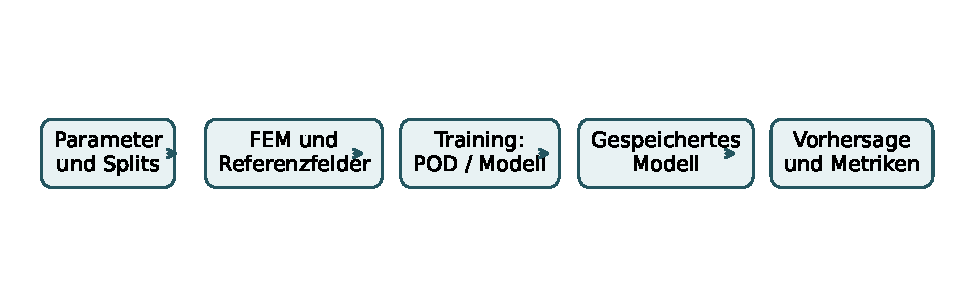
\includegraphics[width=.95\linewidth,height=.66\textheight,keepaspectratio]{figures/architektur.pdf}
\caption{Schematische Daten- und Kontrollwege. Historische und neue Ausführungen besitzen getrennte Artefakte.}\end{figure}
\begingroup\small\begin{longtable}{>{\raggedright\arraybackslash}p{0.400\textwidth}>{\raggedright\arraybackslash}p{0.400\textwidth}}
\toprule
Aufgabe & Tatsächliche Einstiegspunkte\\ \midrule\endhead
Parameter und Einstellungen & config.m, designs/, Studienprotokolle\\
Statische FEM und Datensatz & src/solve\_\allowbreak{}case.m, src/generate\_\allowbreak{}dataset.m\\
Modal-FEM und Vergleich & +femstudy/+fem/modal.m, compareModes.m\\
Modellinventar und Adapter & +femstudy/+models/registry.m, predictLegacy.m\\
Experimente & run\_\allowbreak{}migration\_\allowbreak{}phase1.m, run\_\allowbreak{}hybrid\_\allowbreak{}static\_\allowbreak{}audit.m, run\_\allowbreak{}controlled\_\allowbreak{}gpr\_\allowbreak{}fits.m\\
Metriken & src/field\_\allowbreak{}error.m, +femstudy/+metrics/frequency.m, Diagnoseskripte\\
Dokumentation & gespeicherte MAT-/CSV-Dateien und Berichtsgeneratoren\\
\bottomrule\end{longtable}\endgroup
Am Beispiel des normalisierten Hybridmodells: Das vorab festgelegte Protokoll nennt IDs, Rang und Kernel. Die Trainingsdaten liefern FEM-Felder, Parameter und Gewichte; aus dem Balkenfeld wird das Differenzfeld gebildet. Eine gewichtete POD und GPR-Modelle werden nur auf dem Training angepasst und zusammen mit IDs, Skalen und Parametern gespeichert. controlled\_\allowbreak{}predict.m nimmt das geladene Modell, Parameter und Referenzkoordinaten entgegen, jedoch kein FEM-Zielfeld. Es berechnet Balkenfeld, GPR-Koeffizienten und Rekonstruktion. Erst die getrennte Auswertung vergleicht die Vorhersage mit einem Referenzfeld. Die hier geprüfte Online-Schnittstelle ist eine spezifische Funktion, kein Nachweis für alle historischen Dienste.

\section{5. Modellbestand und Mathematik}
\begingroup\small\begin{longtable}{>{\raggedright\arraybackslash}p{0.200\textwidth}>{\raggedright\arraybackslash}p{0.200\textwidth}>{\raggedright\arraybackslash}p{0.200\textwidth}>{\raggedright\arraybackslash}p{0.200\textwidth}}
\toprule
Verfahren & Ausgabe & Aufbau und Onlinebedarf & Belegter Stand\\ \midrule\endhead
Scalar\_\allowbreak{}GPR & statische Spitze und Gittermaximum & skalare FEM-Ziele; online GPR & historisch vorhanden, Adapter geprüft\\
Beam\_\allowbreak{}theory & statische Spitze & Balkenformel, keine Trainingsdaten & physikalische Baseline, Adapter geprüft\\
Beam\_\allowbreak{}plus\_\allowbreak{}GPR & statische Spitze & Balkenformel plus GPR auf skalarem Rest & historisch vorhanden, Adapter geprüft\\
POD\_\allowbreak{}GP & statisches Feld & Feld-POD und Koeffizienten-GPR & historisch vorhanden, Adapter geprüft\\
POD\_\allowbreak{}RBF & statisches Feld & Feld-POD und RBF-Regressor & historisch vorhanden, Adapter geprüft\\
POD\_\allowbreak{}MLP & statisches Feld & Feld-POD und neuronales Netz & historisch vorhanden, Adapter geprüft\\
POD\_\allowbreak{}Galerkin & statisches Feld & native Basis, Onlineassemblierung und Übertragung & historisch vorhanden, Adapter an einem Fall geprüft\\
DeepONet & statisches Feld an Punkten & trainiertes Parameter-/Ortsnetz & historisch vorhanden, Adapter geprüft\\
Frequency\_\allowbreak{}GPR & sechs sortierte Frequenzen & Modal-FEM-Frequenzen, online GPR und Sortierung & Integration ausgeführt; keine Eigenformen\\
Beam\_\allowbreak{}Field\_\allowbreak{}POD\_\allowbreak{}GPR & statisches Feld & Balkenfeld plus POD-GPR-Rest & implementiert und im kleinen Vergleich untersucht\\
F/E-normalisiert direkt / hybrid & statisches Feld & eigene POD- und GPR-Artefakte, bekannte Parameter & separate Entwicklungsvarianten\\
\bottomrule\end{longtable}\endgroup
\subsection{5.1 Gaußprozessregression und skalare Modelle}
Ein Gaußprozess (GPR) modelliert die gesuchte Funktion probabilistisch. Sein Kernel $k(\mu,\mu')$ beschreibt, wie stark Funktionswerte zweier Eingaben vorab zusammenhängen. Ein großer Längenmaßstab erlaubt einen langsamen Verlauf in dieser Eingaberichtung; unterschiedliche Längen je Parameter heißen ARD. Die trainierte Vorhersage setzt die Ähnlichkeit zum Training und die beobachteten Zielwerte zusammen. Für einen standardisierten Zielwert hat der Mittelwert schematisch die Form

\[\hat a(\mu_*)=m(\mu_*)+k_*^T(K_X+\sigma^2I)^{-1}(a-m_X).\]
$K_X$ enthält Kernelwerte zwischen Trainingsfällen, $k_*$ die Werte zum neuen Fall und $\sigma$ einen Rausch- beziehungsweise Regularisierungsparameter in der jeweiligen standardisierten Zielgröße. Ein Squared-Exponential-Kernel ist sehr glatt; Matérn-5/2 erlaubt eine andere Glattheitsannahme. Kernelparameter werden anhand des Trainings angepasst. Die vom Modell berechnete Unsicherheit hängt von diesen Annahmen ab; sie ist keine garantierte FEM-Fehlerschranke.

Scalar\_\allowbreak{}GPR lernt die Spitzenverschiebung und das Gittermaximum separat. Beam\_\allowbreak{}theory verwendet für einen Euler-Bernoulli-Kragbalken $u_{\rm tip}=F_zL^3/(3EI)$ mit $I=bh^3/12$. Beam\_\allowbreak{}plus\_\allowbreak{}GPR addiert einen aus statischen FEM-Spitzen gelernten skalaren Rest. Es liefert kein vollständiges Feld. Beide Balkenansätze brauchen online Geometrie, $E$ und Last; nur die Korrektur benötigt zuvor trainierte Daten.

\subsection{5.2 POD: aus vielen Feldwerten wenige Koeffizienten}
Eine Proper Orthogonal Decomposition (POD) sucht wiederkehrende räumliche Muster in mehreren Trainingsfeldern. Anschaulich ersetzt sie viele ähnliche Verschiebungsvektoren durch eine gemeinsame mittlere Form und wenige veränderliche Gewichte. Nach Abzug des Trainingsmittelwerts $\bar u$ wird die gewichtete Snapshotmatrix zerlegt:

\[W^{1/2}(S-\bar u\mathbf1^T)=Q\Sigma V^T,\qquad \Phi_r=W^{-1/2}Q_{(:,1:r)}.\]
Eine Näherung hat die Form $u\approx\bar u+\Phi_ra$, wobei $a=\Phi_r^TW(u-\bar u)$ die POD-Koeffizienten sind. Die Basisvektoren sind aus Daten abgeleitete typische Muster, keine mechanischen Eigenformen. Der Projektionsfehler misst, wie gut sich ein bekanntes Referenzfeld mit dieser Basis überhaupt darstellen lässt. Der Vorhersagefehler enthält zusätzlich den Fehler der vorhergesagten Koeffizienten. Ein kleiner Projektionsfehler garantiert daher keine gute Regression.

Bei POD\_\allowbreak{}GP lernt ein separater GPR die Koeffizienten. POD\_\allowbreak{}RBF interpoliert beziehungsweise regularisiert sie mit einer kubischen radialen Basis und linearem Polynom. POD\_\allowbreak{}MLP verwendet ein zweischichtiges neuronales Netz mit tanh-Aktivierung; die Gewichte werden mit Adam angepasst. Anders als beim GPR wird die Funktion hier durch trainierte Netzgewichte dargestellt, nicht durch einen Kernel und eine Kovarianzmatrix der Trainingsfälle. Alle drei benötigen online keine FEM-Lösung.

\subsection{5.3 Galerkin und DeepONet}
Der POD-Galerkin-ROM nutzt ebenfalls eine reduzierte Basis, setzt sie jedoch in die mechanische Gleichung ein. Mit einer passenden nativen Basis $V$ lautet das reduzierte System $V^TK(\mu)Vq=V^Tf(\mu)$ und $u\approx Vq$. Die Koeffizienten folgen somit aus einem reduzierten mechanischen Gleichgewicht statt aus einer rein gelernten Regression. Im vorliegenden Projekt bleiben Online-Matrixassemblierung und räumliche Übertragung relevante Kosten. Die native Basis ist nicht mit der auf Abfragepunkten trainierten POD-Basis gleichzusetzen.

DeepONet verbindet ein Netz für die Parameter mit einem zweiten Netz für den Abfrageort. Schematisch entsteht eine Komponente durch ein Skalarprodukt der beiden Merkmalsvektoren: $\hat u_c(\mu,x)=\sum_j b_{cj}(\mu)t_{cj}(x)$. Die trainierten Gewichte erlauben anschließend ortsabhängige Feldvorhersagen ohne Online-FEM. Die historische Untersuchung nutzte fünf Seeds; im Adaptertest wurde nur Seed 42 betrachtet.

\subsection{5.4 Frequenzmodell und hybrides Korrekturfeld}
Das Frequenz-GPR verwendet Geometrie, Material und Dichte statt statischer Last. Die sechs aufsteigend sortierten Frequenzen werden logarithmiert und getrennt mit je einem GPR gelernt. Die Exponentialfunktion stellt positive Vorhersagen sicher. Auf der Validierung wird zwischen zwei trainierten Kernelkandidaten gewählt; der gewählte Kandidat wird ohne Validierungs- oder Testnachtraining eingefroren. Die anschließende Sortierung nutzt keine FEM-Testwerte. Sie ordnet Spektralwerte, verfolgt aber keine physikalischen Modenfamilien.

Das statische Balkenfeld verwendet Euler-Bernoulli-Kinematik mit axialer Biegerotation und transversaler Durchbiegung. $u_y=0$, Schubverformung und Querschnittsverwölbung sind nicht erfasst. Im hybriden Modell wird das Differenzfeld $\Delta u=u_{\rm FEM}-u_{\rm Balken}$ durch eine eigene gewichtete POD komprimiert. Die Onlinevorhersage ist $\hat u=u_{\rm Balken}+\overline{\Delta u}+\Phi_{\Delta}\hat a_{\Delta}$. Im Vergleich zum direkten POD-Modell lernt die Regression also die verbleibende Korrektur statt des gesamten Feldes. Rohfeld und gegebenenfalls nachträglich auf null gesetzte Einspannung müssen getrennt bewertet werden.

Die spätere Normierung verwendet die aus linearer Statik bekannte Skalierung $s=(F_z/F_{\rm ref})(E_{\rm ref}/E)$ mit $F_{\rm ref}=-500$ N und $E_{\rm ref}=10^{11}$ Pa. Trainingsvollfelder beziehungsweise Differenzfelder werden durch $s$ geteilt; die Vorhersage wird wieder mit $s$ multipliziert. $s$ ist dimensionslos. Dies setzt gleiche Lastform und lineares Verhalten voraus; Geometrie und $\nu$ bleiben variabel. Die implementierte Schnittstelle akzeptiert für diesen Versuch nur $F_z<0$ und $E>0$ und weist $F_z=0$ ab.

\section{6. Datentrennung und Auswahl}
Ein Trainingsfall passt Modellparameter und Vorverarbeitung an. Die Validierung dient Entwicklungs- oder Auswahlentscheidungen. Ein unabhängiger Test darf erst nach Einfrieren der Entscheidungen beurteilt werden. Werden Fälle mehrfach für Diagnosen und Modellwahl betrachtet, sind sie Entwicklungsdaten und keine neue blinde Bestätigung.

\begingroup\small\begin{longtable}{>{\raggedright\arraybackslash}p{0.200\textwidth}>{\raggedright\arraybackslash}p{0.200\textwidth}>{\raggedright\arraybackslash}p{0.200\textwidth}>{\raggedright\arraybackslash}p{0.200\textwidth}}
\toprule
Reihe & Training & Validierung & Test / Verwendung\\ \midrule\endhead
Historische Statik & verschachtelt 12, 24, 48, 96, 192, 384; bei 384 IDs 1–12 und 25–396 & 13–18 & 19–24, mehrfach betrachtet\\
Modal-Integration & 1–12 & 13–18 & 19–24, kleiner Integrationsvergleich\\
Eingefrorener Hybridvergleich & 1–12 und 25–30, insgesamt 18 & 31–36 & 19–24 erst nach Auswahl; historisch bereits betrachtet\\
Kontrollierte Folge-Fits & gleiche 18 & gleiche sechs, wiederholt für Entwicklung verwendet & historische Testfälle nicht ausgewertet\\
\bottomrule\end{longtable}\endgroup
Die ursprünglichen Kandidaten des eingefrorenen Hybridvergleichs umfassten POD-Ränge 1, 2, 4, 8 und 12 sowie Matérn-5/2 und Squared-Exponential; der mittlere relative Validierungsfeldfehler wählte zwischen den Kandidaten einschließlich der reinen Balkenbaseline. Für die späteren Diagnose-Fits waren Rang 2 direkt und Rang 4 hybrid fest. Jeweils drei vorab festgelegte Kernelstarts mit festem und drei mit lernbarem Sigma wurden innerhalb ihrer Gruppe nach Trainings-Log-Likelihood ausgewählt. Die zusätzliche normierte Variante ist ein eigener Entwicklungsschritt. Seed 42 ist keine Wiederholungsstudie; die historische DeepONet-Reihe ist eine gesonderte fünf-Seed-Auswertung.

Der getrennte Entwurf einer größeren Modalstudie sieht als Planungsvorschlag bis zu 384 bisherige Trainingsfälle und zusätzlich je 64 neue unabhängige Validierungs- und Testfälle vor. Ein Teil des möglichen Datenbedarfs ist noch nicht auditiert; die vorgeschlagenen neuen Fälle wurden nicht erzeugt und die große Lernkurve wurde nicht gestartet. Die historische Nutzung eines Falles zum Training schließt seine nachträgliche Verwendung als unabhängigen Test aus.

\section{7. Historische statische Lernkurve}
Die folgende Tabelle übernimmt historische Medianwerte aus experiments/deeponet\_\allowbreak{}20261023\_\allowbreak{}v1/REPORT.md und dem früheren Gesamtbericht. Eine separate Nachberechnung aller historischen Kennzahlen wurde für diese Ausarbeitung nicht durchgeführt. Bei DeepONet ist die Aggregation ein Median über fünf Seed-Mediane; bei den älteren POD-Regressoren ist eine solche Seed-Streuung hier nicht belegt.

\begingroup\small\begin{longtable}{>{\raggedright\arraybackslash}p{0.160\textwidth}>{\raggedright\arraybackslash}p{0.160\textwidth}>{\raggedright\arraybackslash}p{0.160\textwidth}>{\raggedright\arraybackslash}p{0.160\textwidth}>{\raggedright\arraybackslash}p{0.160\textwidth}}
\toprule
Trainingsfälle & POD-GPR & POD-RBF & POD-MLP & DeepONet\\ \midrule\endhead
12 & 60,652 & 23,258 & 21,458 & 45,756\\
24 & 23,247 & 26,307 & 9,851 & 52,130\\
48 & 4,656 & 18,409 & 13,374 & 43,260\\
96 & 3,497 & 5,406 & 13,799 & 31,177\\
192 & 1,144 & 3,636 & 8,109 & 10,429\\
384 & 0,384 & 5,459 & 3,314 & 8,835\\
\bottomrule\end{longtable}\endgroup
Alle Zahlen sind Prozent relativer gewichteter Gesamtfeldfehler auf denselben sechs historischen Testfällen. Der historische POD-Galerkin-ROM erreicht bei 384 Fällen einen Median von ungefähr 0,057 \%, nutzt aber ein anderes gemeinsames FEM-Netz und Onlineassemblierung. Historisch dokumentierte Medianzeiten lagen bei ungefähr 914,7 ms ROM und 3,05 ms POD-GPR; dies sind frühere Einzelmessbedingungen und kein kontrollierter universeller Geschwindigkeitsvergleich.

\begin{figure}[H]\centering
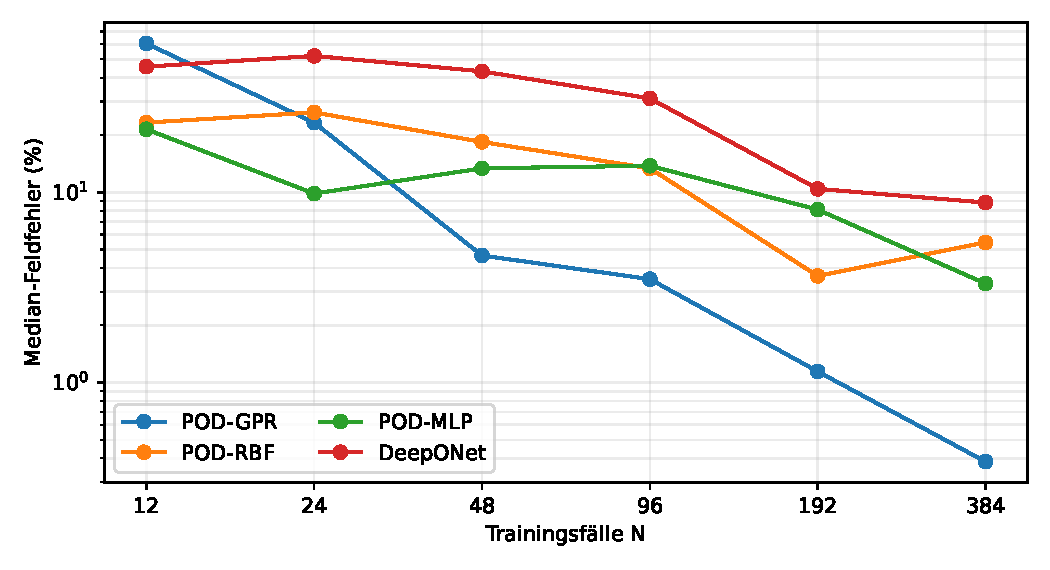
\includegraphics[width=.95\linewidth,height=.66\textheight,keepaspectratio]{figures/lernkurve.pdf}
\caption{Historische statische Lernkurven: Median über sechs Testfälle; DeepONet zusätzlich Median über fünf Seed-Mediane. Quelle: früherer Projektbericht.}\end{figure}
\begin{figure}[H]\centering
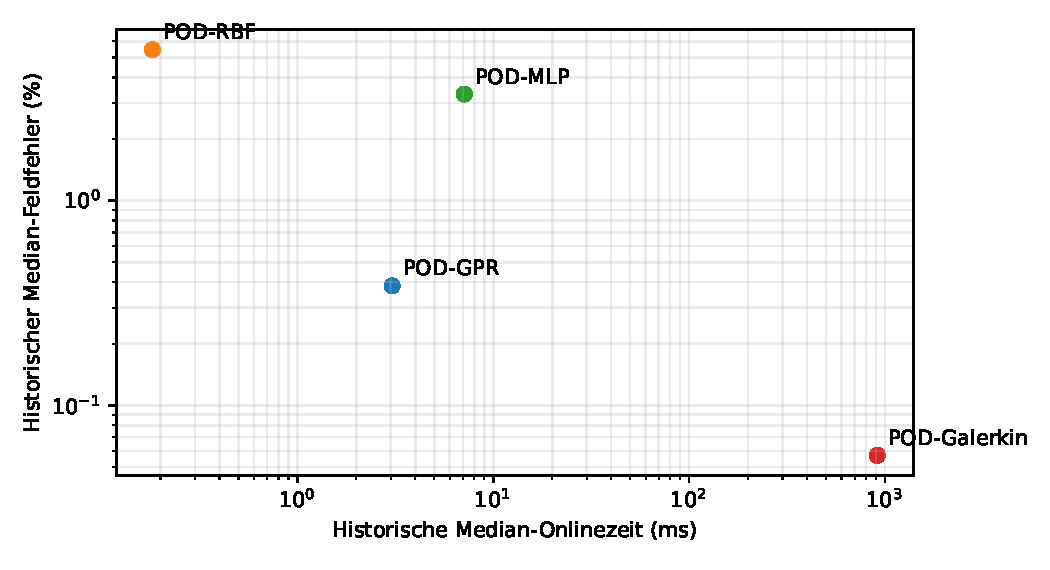
\includegraphics[width=.95\linewidth,height=.66\textheight,keepaspectratio]{figures/kosten.pdf}
\caption{Historischer Vergleich bei N=384: Medianfeldfehler und separat berichtete Median-Onlinezeit. Unterschiedliche Onlineoperationen und Netzräume begrenzen die Vergleichbarkeit; Quelle frühere Berichte.}\end{figure}
\section{8. Architekturmigration und Modal-Integrationslauf}
Im Adaptervergleich wurden für sieben vorhandene Verfahren sechs Fälle und für den ROM ein Fall über alte und neue Aufrufe verglichen. Die maximalen Differenzen waren jeweils null. Das prüft die Weiterleitung dieser Aufrufe, nicht alle historischen Kennzahlen. Ein kleiner Scalar-GPR wurde separat als Schnittstellenprobe trainiert.

Vor der kleinen modalen Datenerzeugung wurden die Fälle 1, 6 und 12 auf drei quadratischen Netzstufen mit $H_{\max}=\min(b,h)/2$, /3 und /4 untersucht. Die größte Änderung unter den sechs zugeordneten Zielfrequenzen von /3 zu /4 betrug 0,11985 \%, 0,17847 \% und 0,10615 \%. Alle drei Ergebnisse bestanden das vorläufige 2-\%-Kriterium. Dies belegt die untersuchten Kombinationen, nicht den gesamten Parameterraum. Die Modenzuordnung verwendet gewichtete Ähnlichkeiten auf dem übertragenen Gitter. Die 1-\%-Abstandsregel ist eine konfigurierbare Clusterheuristik; Unterräume, Rang und Pufferränder werden berücksichtigt. Eine Warnung zur Eckknoten-Triangulation bei quadratischen Mittelknoten ist dokumentiert und bleibt eine Grenze der Übertragungsprüfung.

Die zusätzliche Dichteprüfung verdoppelte $\rho$ bei gleichem Netz von 7850 auf 15700 kg/m³. Die größte relative Abweichung vom erwarteten Faktor $1/\sqrt2$ betrug $1{,}7355\cdot10^{-9}$. Diese geänderte Dichte gehört zum Test, nicht zum eigentlichen Studiensplit.

\begin{figure}[H]\centering
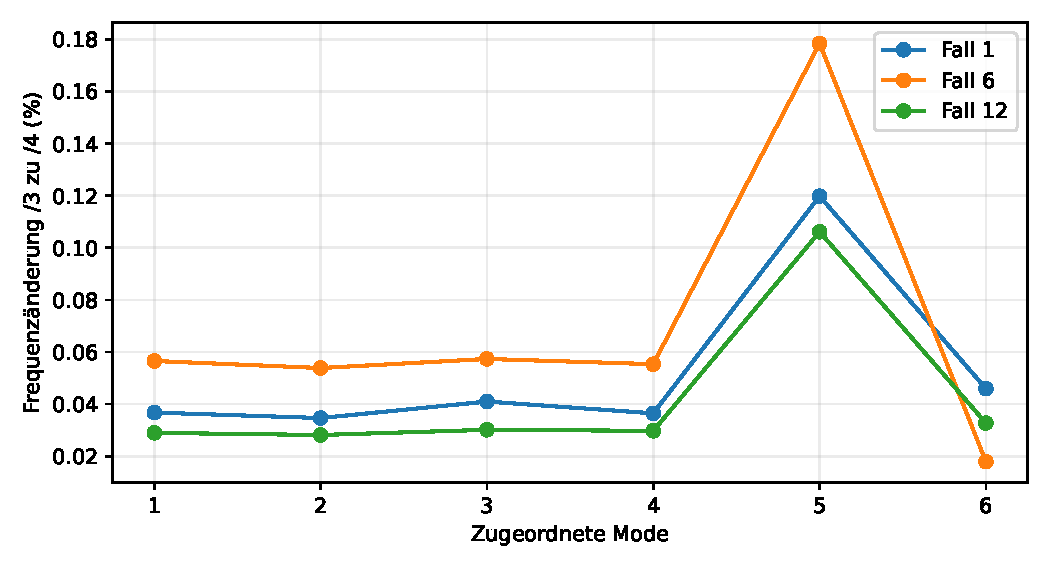
\includegraphics[width=.95\linewidth,height=.66\textheight,keepaspectratio]{figures/modal_netz.pdf}
\caption{Modal-Netzprüfung: maximale Frequenzänderung unter sechs Moden zwischen den beiden feinsten Stufen, drei Parameterfälle; Quelle comparison\_\allowbreak{}*.mat.}\end{figure}
Für den Frequenz-GPR lagen die mittleren Validierungsfehler bei 8,163 \% für Matérn-5/2 und 3,856 \% für Squared-Exponential. Letzterer wurde gewählt. Der mittlere Fehler auf den sechs Testfällen betrug vor und nach der Sortierung 3,366 \%; es gab keine Reihenfolgeverletzung. Für die Moden 1 bis 6 waren die mittleren Fehler 1,810 \%, 3,050 \%, 1,668 \%, 5,595 \%, 3,687 \% und 4,386 \%. Jede Zahl beruht auf denselben sechs Fällen, nicht auf sechs weiteren unabhängigen Versuchen.

\begin{figure}[H]\centering
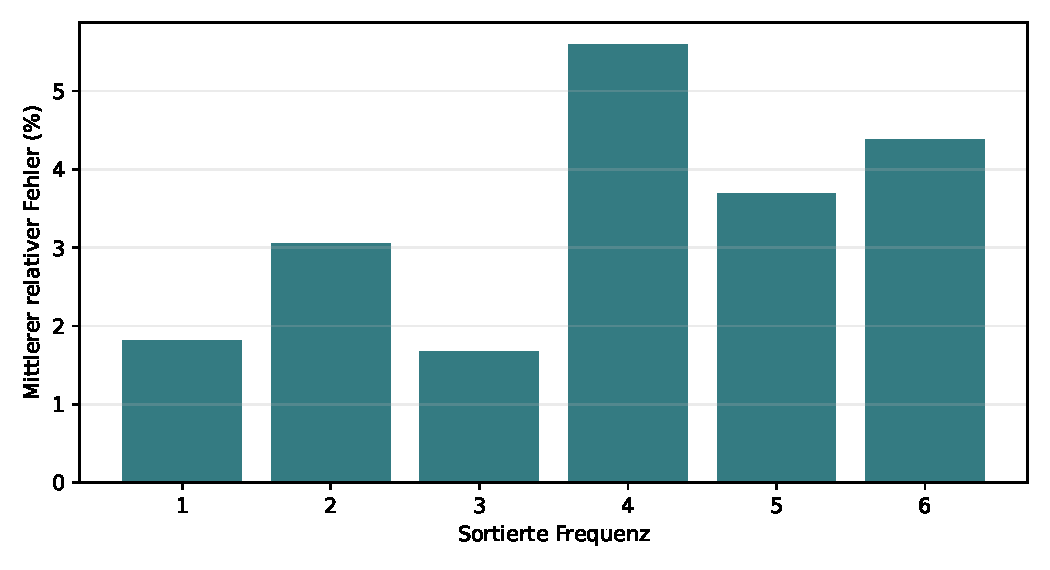
\includegraphics[width=.95\linewidth,height=.66\textheight,keepaspectratio]{figures/modal_fehler.pdf}
\caption{Mittlerer relativer Frequenzfehler je sortierter Mode über sechs historische Testfälle; Quelle frequency\_\allowbreak{}evaluation.mat.}\end{figure}
\section{9. Eingefrorener statischer Hybridvergleich}
Für 18 Trainings- und sechs interne Validierungsfälle wurde vor der historischen Testauswertung zwischen reinem Balken, direktem und hybridem POD-GPR gewählt. Die auf der Validierung gewählten POD-Kandidaten hatten Rang 2 direkt und Rang 4 hybrid, jeweils Squared-Exponential. Nach der vorab festgelegten Regel gewann das Balkenfeld.

\begingroup\small\begin{longtable}{>{\raggedright\arraybackslash}p{0.200\textwidth}>{\raggedright\arraybackslash}p{0.200\textwidth}>{\raggedright\arraybackslash}p{0.200\textwidth}>{\raggedright\arraybackslash}p{0.200\textwidth}}
\toprule
Split und Kennwert & Balken & Direktes POD-GPR & Hybrid\\ \midrule\endhead
Training: Mittel / Median / Maximum & 0,590 / 0,461 / 1,836 \% & 0,0550 / 0,0443 / 0,1628 \% & 0,00472 / 0,00277 / 0,02696 \%\\
Validierung: Mittel / Median / Maximum & 0,5215 / 0,4620 / 0,8698 \% & 113,834 / 36,711 / 347,857 \% & 0,8544 / 0,5462 / 2,6836 \%\\
Historischer Test: Mittel / Median / Maximum & 0,6563 / 0,4626 / 1,7197 \% & 67,828 / 32,244 / 255,707 \% & 0,7359 / 0,1785 / 2,3117 \%\\
\bottomrule\end{longtable}\endgroup
Die Daten stammen aus diagnostics\_\allowbreak{}v1.mat und dem zugehörigen Diagnosebericht. Der Test war schon historisch betrachtet. Trotz günstigerem Testmedian war das Hybridmodell in zwei der sechs Fälle schlechter als das Balkenfeld; Mittelwert und Median erzählen daher unterschiedliche Teile der Geschichte. Ein einzelner großer Fall kann den Mittelwert stark beeinflussen, während der Median die mittlere Position der sortierten Fallwerte beschreibt.

\begin{figure}[H]\centering
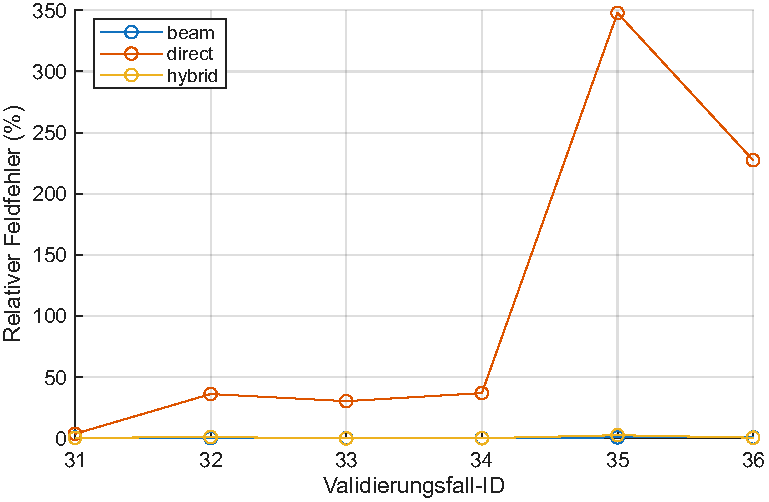
\includegraphics[width=.95\linewidth,height=.66\textheight,keepaspectratio]{figures/validation_case_errors.pdf}
\caption{Fallweise Fehler der eingefrorenen Kandidaten auf sechs internen Validierungsfällen; Quelle diagnostics\_\allowbreak{}v1.mat.}\end{figure}
\section{10. Ursachenanalyse und kontrollierte Folge-Fits}
Die direkte POD hatte auf der internen Validierung einen mittleren Projektionsfehler von 0,0654 \%, bei 113,834 \% Vorhersagefehler. Beim Hybrid betrugen die entsprechenden Werte 0,01185 \% und 0,8544 \%. Die vorhandene Basis kann die betrachteten Felder also deutlich besser darstellen, als die gelernten Koeffizienten sie vorhersagen. Daraus folgt keine allgemeine Fehlerfreiheit der Regression. Die gewichtete Orthonormalität $\Phi^TW\Phi\approx I$ wich in Frobeniusnorm um 8,08·$10^{-16}$ beziehungsweise 2,98·$10^{-15}$ ab.

\begin{figure}[H]\centering
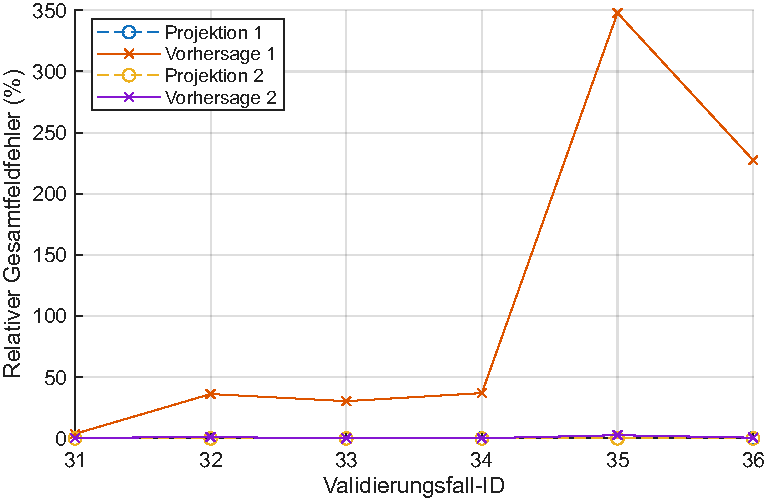
\includegraphics[width=.95\linewidth,height=.66\textheight,keepaspectratio]{figures/projection_vs_prediction.pdf}
\caption{Vergleich von Projektion und Vorhersage der eingefrorenen direkten und hybriden Modelle, sechs interne Validierungsfälle; Quelle diagnostics\_\allowbreak{}v1.mat.}\end{figure}
Die gespeicherten Trainingsmittelwerte und Standardabweichungen der Koeffizienten stimmen mit der getrennten Nachrechnung überein. Die manuelle GPR-Berechnung reproduzierte die standardisierten MATLAB-Vorhersagen aller geprüften Koeffizienten mit maximal 2,84·$10^{-14}$ Abweichung. Die Validierungsfälle haben minimale Abstände von 1,48 bis 2,66 im train-only standardisierten Eingaberaum; drei liegen außerhalb mindestens eines einzelnen Trainingsintervalls. Gute einzelne Intervallabdeckung ist keine Garantie für gemeinsame Abdeckung.

Bei der ersten Kernelkorrelationsdiagnose wurde ein Kernelname wegen Groß-/Kleinschreibung falsch erkannt. Die Korrelationen aus analysis.mat sind ungültig; maßgeblich ist analysis\_\allowbreak{}v2.mat. Dort liegt für den ersten direkten Koeffizienten die maximale Korrelation zum Training zwischen 0,754 und 0,973. Eine pauschale Erklärung durch verschwindende Korrelationen ist damit nicht belegt. Der Fehler betraf die Diagnoseroutine, nicht die eingefrorenen Vorhersagen. Ein erster synthetischer Koeffiziententest hatte außerdem einen falsch transponierten Erwartungswert; nach Korrektur des Erwartungswerts bestand der Test.

\begin{figure}[H]\centering
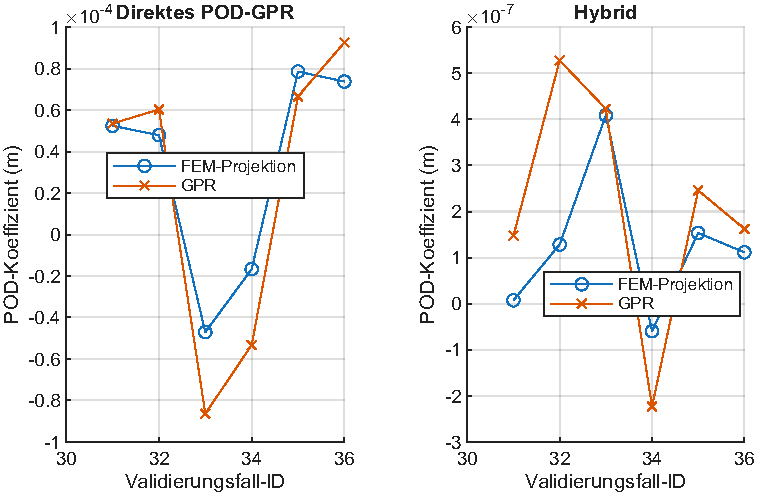
\includegraphics[width=.95\linewidth,height=.66\textheight,keepaspectratio]{figures/validation_coefficients.pdf}
\caption{Tatsächliche und vorhergesagte POD-Koeffizienten der eingefrorenen Modelle auf der internen Validierung; Quelle diagnostics\_\allowbreak{}v1.mat.}\end{figure}
Die kontrollierten Folge-Fits wurden vor Ausführung festgelegt und in eigenen Dateien gespeichert. Die Kontrollwiederholung des direkten Modells reproduzierte die alten Validierungsfelder exakt; die ursprüngliche Initialisierung war nicht vollständig protokolliert. Andere Starts und lernbares Sigma verbessern den Validierungsmittelwert praktisch nicht. MATLAB meldete bei lernbarem Sigma, dass der Initialwert zu nahe an der Untergrenze lag, und hob ihn an. Die gespeicherten Warnungen sind Teil des Ergebnisses; vollständige Optimierungsabbruchinformationen waren nicht verfügbar.

\begingroup\small\begin{longtable}{>{\raggedright\arraybackslash}p{0.267\textwidth}>{\raggedright\arraybackslash}p{0.267\textwidth}>{\raggedright\arraybackslash}p{0.267\textwidth}}
\toprule
Modell / Entwicklungskandidat & Mittlerer Validierungsfehler & Mittlerer Projektionsfehler\\ \midrule\endhead
Balken & 0,5215 \% & —\\
Direkt, Kontrolle & 113,834 \% & 0,0654 \%\\
Direkt, bester fester Start nach Trainingsziel & 113,835 \% & 0,0654 \%\\
Direkt, lernbares Sigma nach Trainingsziel & 113,808 \% & 0,0654 \%\\
Direkt, F/E-normalisiert & 10,687 \% & 0,0488 \%\\
Hybrid, Kontrolle & 0,8544 \% & 0,01185 \%\\
Hybrid, bester fester Start nach Trainingsziel & 0,8544 \% & 0,01185 \%\\
Hybrid, lernbares Sigma nach Trainingsziel & 0,8544 \% & 0,01185 \%\\
Hybrid, F/E-normalisiert & 0,1289 \% & 0,00443 \%\\
\bottomrule\end{longtable}\endgroup
Quelle: fit\_\allowbreak{}summary.csv und einzelne fit\_\allowbreak{}*.mat. Die Normierung verändert sowohl die POD-Basis als auch die Regression und kann daher nicht als isolierter Nachweis einer einzigen Ursache interpretiert werden. Kleine Trainingsfehler belegen zunächst nur die Anpassung an die bereits gesehenen Fälle. Die wiederholt betrachteten sechs Validierungsfälle sind für eine unabhängige Bestätigung ungeeignet.

\begin{figure}[H]\centering
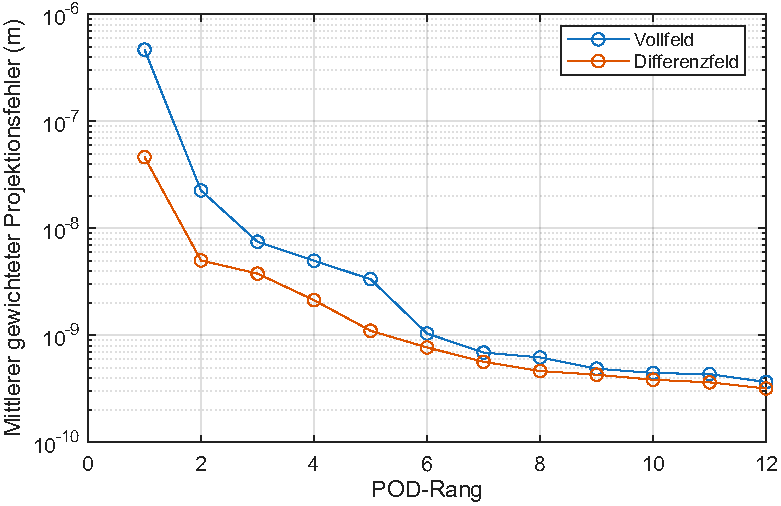
\includegraphics[width=.95\linewidth,height=.66\textheight,keepaspectratio]{figures/pod_compression.pdf}
\caption{Komprimierungsvergleich: absoluter gewichteter Projektionsfehler von Voll- und Differenzfeld auf derselben physikalischen Skala, interne Validierung; Quelle gespeicherte Trainings- und Validierungsfelder.}\end{figure}
\begin{figure}[H]\centering
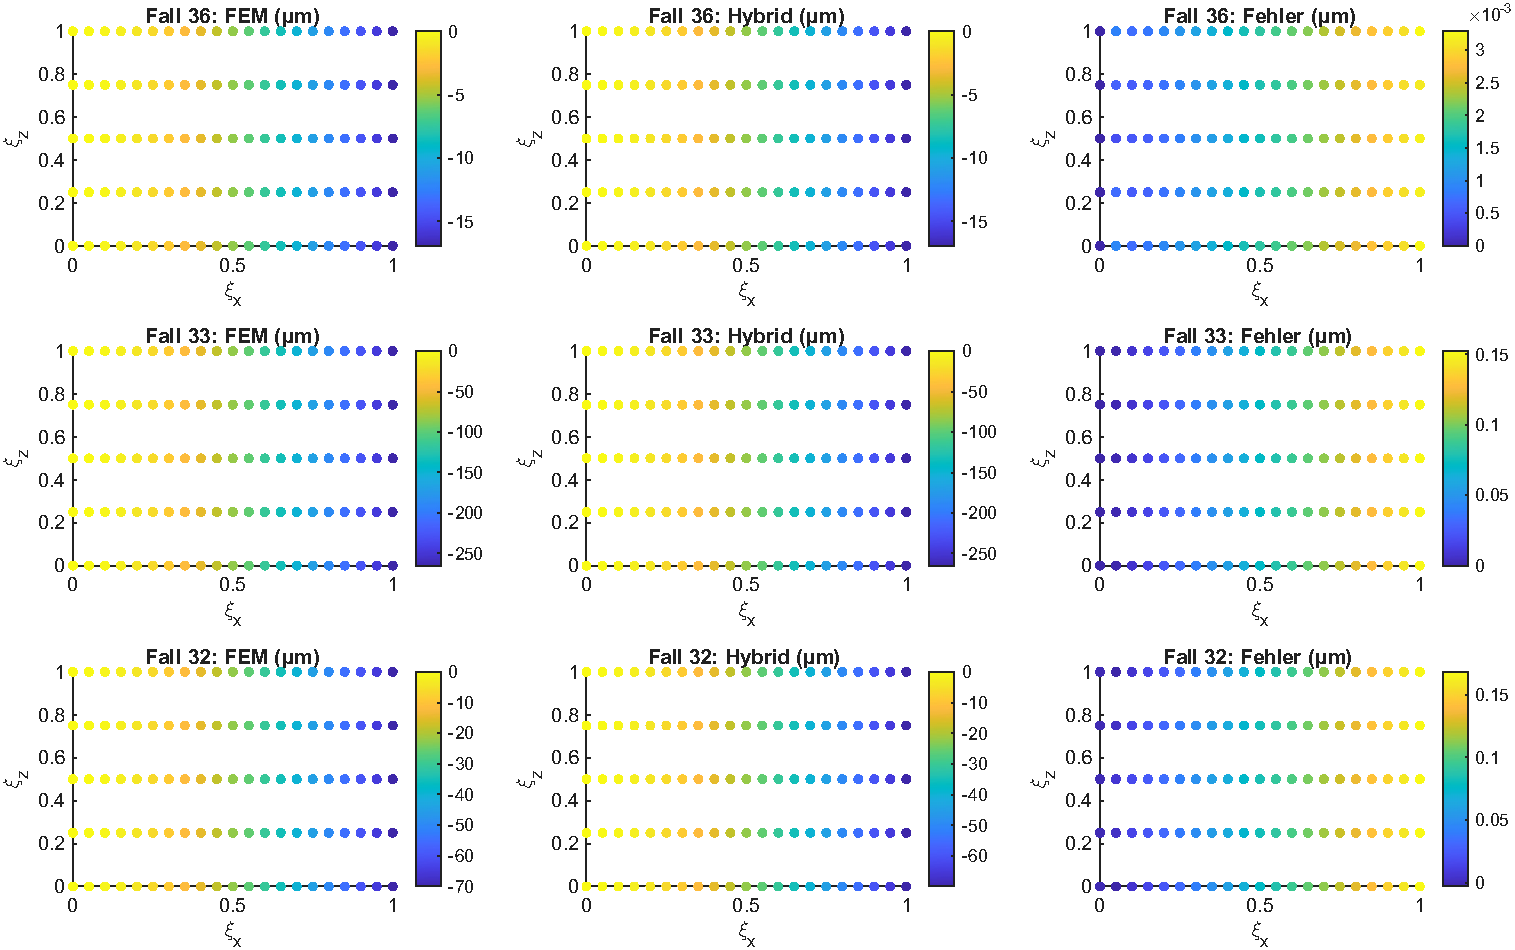
\includegraphics[width=.95\linewidth,height=.66\textheight,keepaspectratio]{figures/field_cases.pdf}
\caption{Repräsentative FEM-, Hybrid- und Fehlerfelder der normierten Variante für drei interne Validierungsfälle; Quelle gespeicherte Felder.}\end{figure}
\section{11. Diskussion und Geltungsbereich}
Das reine Balkenmodell ist in dieser speziellen Aufgabe stark, weil Geometrie, Einspannung und Last der Balkenannahme nahestehen. Sein Erfolg ist keine allgemeine Aussage über komplexe Bauteile. Ein Korrekturmodell muss zunächst eine bereits kleine physikalische Restabweichung zuverlässig vorhersagen; es kann sie bei einzelnen Fällen auch vergrößern.

Relative Komponentenfehler können groß werden, wenn die zugehörige Referenzkomponente nahezu null ist. Absolute Fehler in Metern und eine explizite Nahe-null-Regel ergänzen deshalb die relativen Werte. Vergleichbare Aggregationen sind Voraussetzung jeder Rangfolge: Mittel und Median, sechs Fälle und fünf Seeds sowie direkte Regression und Online-ROM dürfen nicht stillschweigend vermischt werden.

Ein dokumentiertes historisches Beispiel ist die kleine $u_y$-Komponente von DeepONet bei N=384: Der frühere Bericht nennt für 30 Seed-Fall-Kombinationen einen Median des relativen Komponentenfehlers von 1466,17 \%, während der zugehörige Median des absoluten gewichteten RMS-Fehlers etwa 0,858 Mikrometer betrug. Beide Größen beschreiben denselben Befund aus unterschiedlicher Perspektive; ein großer relativer Wert allein legt die absolute Größenordnung nicht fest. Quelle ist der frühere DeepONet-Bericht, nicht eine neue Nachrechnung.

Die beobachtete Verbesserung der normierten Varianten ist ein plausibler Hinweis, dass die bekannte Last-/Steifigkeitsstruktur bei kleiner Stichprobe nützlich ist. Sie beweist weder eine eindeutige Fehlerursache noch Robustheit außerhalb der Entwicklungsdaten. Die geprüften anderen Startwerte und Sigma-Einstellungen schließen nicht alle denkbaren Optimierungsprobleme aus. Auch die GPR-Unsicherheit bleibt eine modellabhängige Aussage und muss mit unabhängigen Referenzen geprüft werden.

Statischer Feldfehler und Frequenzfehler messen unterschiedliche Größen. Die Modalvalidierung erlaubt zudem keine Aussage über gelernte Eigenformen. Nahe oder mehrfache Eigenwerte erschweren eine Einzelmodenzuordnung; hier ist der Vergleich geeigneter Unterräume sinnvoller. Die bisherigen Modalnetz- und Clustertests sind zu klein, um alle Grenzfälle oder die Übertragbarkeit auf andere Geometrien zu beweisen.

\section{12. Fazit und priorisierter Ausblick}
Die vorhandenen Studien zeigen, dass datengetriebene POD-Modelle bei wachsendem Trainingsbestand auf dem hier betrachteten Balken gute Feldfehler erreichen können. Der physikalische Balken ist bei kleinem Budget eine starke Baseline. Das normierte Hybridmodell verbessert die wiederholt betrachtete interne Validierung, aber ein unabhängiger Test steht aus. Der ROM erzielt historisch einen kleinen Fehler bei zusätzlichem mechanischem Onlineaufwand. Das Modal-GPR ist als kleiner Spektral-Integrationslauf belegt; Eigenform-Surrogate sind nicht vorhanden.

Priorität 1 ist eine vorab definierte unabhängige Bewertung eingefrorener normierter Varianten mit neuen, disjunkten Parameterfällen und FEM-Referenzen. Priorität 2 ist die technische Absicherung von Checkpoint-Integrität, vollständiger Schema- und Operatorraumprüfung sowie der noch fehlenden Optimierungsinformationen. Priorität 3 ist erst danach die Entwicklung und Prüfung modaler Hybridmodelle inklusive zuverlässiger Familien- und Clusterbehandlung. Eine Übertragung auf komplexere Strukturen wie einen Elektromotor folgt erst nach einer neuen Problem-, Daten- und Validierungsdefinition.

\section{Anhang A. Prüfverzeichnis}
Die Tabelle bezeichnet den Herkunftsstand. Historisch bedeutet aus vorliegenden Protokollen übernommen; dokumentarische Nachprüfung bedeutet für diese Ausarbeitung ausschließliches Lesen gespeicherter Artefakte. Kein neuer physikalischer Lauf wurde gestartet.

\begingroup\small\begin{longtable}{>{\raggedright\arraybackslash}p{0.267\textwidth}>{\raggedright\arraybackslash}p{0.267\textwidth}>{\raggedright\arraybackslash}p{0.267\textwidth}}
\toprule
Prüfung / Zweck und Eingaben & Erwartung und Toleranz & Ergebnis, Status und Beleg\\ \midrule\endhead
Kraft, E und Vorzeichen, Balkenfeld & Skalierung; absolut 1e-14 m & historisch bestanden; PRUEFSTAND.md, Einzelprotokoll fehlt\\
Analytische Balkenspitze und Einspannung & Übereinstimmung mit Balkenformel / Null & historisch erwähnt; hybrid\_\allowbreak{}beam\_\allowbreak{}phase1\_\allowbreak{}v1/STATUS.md, Einzeltoleranz nicht vollständig archiviert\\
Einspannung vorher / nachher & rohes Feld und explizites Nullsetzen getrennt & Validierung roh maximal 2,73e-18 m direkt, 1,06e-20 m hybrid; danach null; diagnostics\_\allowbreak{}v1.mat\\
Modalnetz: Fälle 1, 6, 12 & sechs Moden, feinste Stufen <=2 \% und gültige Zuordnung & 0,11985 / 0,17847 / 0,10615 \%; Nachprüfung comparison\_\allowbreak{}*.mat\\
Dichteskalierung gleicher Fall und Netz & Frequenzfaktor 1/sqrt(2) & max. relative Abweichung 1,7355e-9; Nachprüfung density\_\allowbreak{}check.mat\\
Modenübertragung / Cluster & kompatibler Raum, Rang, Pufferrand & drei Netzvergleiche bestanden; Warnung und begrenzter Stichprobenumfang bleiben; compareModes.m\\
Synthetische Vorzeichen-/Clusterrotation & invariantes Vergleichsergebnis & historischer Unit-Test bestanden; tests/test\_\allowbreak{}migration\_\allowbreak{}phase1.m\\
POD-Orthonormalität & $\Phi^TW\Phi=I$ & 8,08e-16 und 2,98e-15 Frobeniusabweichung; diagnostics\_\allowbreak{}v1.mat\\
Encode / Decode, Projektion & trainierte Basis reproduziert Projektion & Projektionsfehler ausdrücklich nicht null; diagnostics\_\allowbreak{}v1.mat; kein allgemeiner Beweis\\
Eingabe-/Ausgabeskalen & nur Training; gespeicherte Werte gleich Nachrechnung & Abweichung null für geprüfte Modelle; analysis\_\allowbreak{}v2.mat, diagnostics\_\allowbreak{}v1.mat\\
Manuelle GPR-Auswertung & Gleichheit zu MATLAB & maximal 2,84e-14 standardisiert; analysis\_\allowbreak{}v2.mat\\
Kernelkorrelation & korrekter Kernelname & erste Diagnose fehlerhaft, v2 korrigiert; BEFUNDE.md, analysis\_\allowbreak{}v2.mat\\
Synthetischer Koeffiziententest & erwartete Rekonstruktion & Erwartungswert erst falsch transponiert, korrigiert und bestanden; BEFUNDE.md\\
Kontrollwiederholung direkt & gespeicherte Validierungsfelder; 1e-12 m & max. 0 m; fit\_\allowbreak{}1\_\allowbreak{}1.mat, ABNAHME.md\\
Starts und Sigma & vorab definierte Starts; Gruppenauswahl Trainingsziel & 16 Kandidaten erfolgreich, Sigma-Warnungen erfasst; PROTOKOLL.md, fit\_\allowbreak{}*.mat\\
F/E-Normierung & bekanntes $F,E$; F=0 abweisen & zwei Varianten ausgeführt, negative Tests bestanden; acceptance.mat\\
Adapter gegen direkte Aufrufe & gleiche Eingaben, gleiche Ausgabe & sechs Fälle für sieben Modelle, ein ROM-Fall; Differenz 0; static\_\allowbreak{}integration.mat\\
Laden und Vorhersage & Differenz <1e-12 m & direkt und hybrid 0 m; acceptance.mat\\
Split und Duplikate & disjunkte IDs und unterschiedliche Parameterzeilen & 18/6/6 geprüft; protocol.mat, DIAGNOSE.md\\
Raum und Schema & abweichende Koordinate / leere Struktur abweisen & bestanden für neue Schnittstelle; run\_\allowbreak{}controlled\_\allowbreak{}acceptance.m\\
Vorhersage ohne FEM-Ziele & Schnittstelle Modell, Parameter, Raum & drei Argumente; bestanden für controlled\_\allowbreak{}predict.m, kein Ganzprogrammbeweis\\
Unterbrechung / Wiederaufnahme & Checkpoint unverändert und zweiter erzeugt & gezielter Zwei-Fit-Test bestanden; resume\_\allowbreak{}check/resume\_\allowbreak{}evidence.mat; kein Hash\\
Berichtsexport & gespeicherte Daten ohne FEM oder Training & ausgeführt; keine instrumentierte Aufrufüberwachung; ABNAHME.md\\
LaTeX / Sichtprüfung & erfolgreiche Kompilierung, lesbare Seiten & neuer Bericht: siehe Prüfprotokoll; frühere Berichte historisch geprüft\\
Allgemeine Checkpointintegrität & Integrität und Herkunft aller gespeicherten Zustände & offen; keine allgemeine Hashprüfung\\
Optimierungsabbruch & vollständiger Fitverlauf & offen; MATLAB-Schnittstelle stellt ihn hier nicht vollständig bereit\\
\bottomrule\end{longtable}\endgroup
\section{Anhang B. Laufzeiten, Dateien und Reproduktion}
Die neu gemessenen Onlinezeiten gelten für MATLAB R2025b Update 1, Windows PCWIN64, AMD Ryzen 5 4500U, sechs Fälle pro Batch, einen Warm-up und fünf Wiederholungen. Für das normalisierte direkte Modell wurden im Mittel etwa 4,8 ms, für das Hybrid 4,7 ms Gesamtzeit gemessen. Beim Hybrid entfielen etwa 1,0 ms auf das Balkenfeld, 2,6 ms auf GPR, 0,4 ms auf Rekonstruktion und 0,2 ms auf Nachbearbeitung; die direkte Berechnung an Referenzpunkten benötigt keine zusätzliche Übertragung. Die Gesamtzeit enthält auch Prüfungen. Messrauschen und Rundung erlauben keine Interpretation kleiner Differenzen. Primärbeleg: experiments/hybrid\_\allowbreak{}controlled\_\allowbreak{}fits\_\allowbreak{}v1/acceptance.mat.

Weitere Primärdateien sind selection.mat, diagnostics\_\allowbreak{}v1.mat, analysis\_\allowbreak{}v2.mat, fit\_\allowbreak{}*.mat, all\_\allowbreak{}cases.csv, all\_\allowbreak{}aggregates.csv, frequency\_\allowbreak{}model.mat, frequency\_\allowbreak{}evaluation.mat und comparison\_\allowbreak{}*.mat. Historische Lernkurvenzahlen und einige ältere Testnachweise wurden aus früheren Berichten übernommen; sie wurden für dieses Dokument nicht unabhängig neu gerechnet.

Der Berichtsgenerator build\_\allowbreak{}synthesis.py liest ausschließlich diese Markdown-Quelle und vorhandene Abbildungen beziehungsweise gespeicherte Ergebnisdateien; er startet keine FEM oder Modelltrainings. Im Dokumentordner wird python build\_\allowbreak{}synthesis.py ausgeführt, danach zweimal lualatex -interaction=nonstopmode -halt-on-error -no-shell-escape ausarbeitung.tex. Die Kopien der verwendeten Abbildungen und ihre Herkunft stehen im Generator. Einzelwerte der kontrollierten Fits sind in den CSV-Dateien und MAT-Artefakten verfügbar.

\section{Anhang C. Symbolverzeichnis und Literatur}
\begingroup\small\begin{longtable}{>{\raggedright\arraybackslash}p{0.267\textwidth}>{\raggedright\arraybackslash}p{0.267\textwidth}>{\raggedright\arraybackslash}p{0.267\textwidth}}
\toprule
Symbol & Bedeutung & Einheit\\ \midrule\endhead
$\mu$ & Parametervektor & gemischt\\
$u,\hat u$ & Referenz- und Vorhersageverschiebung & m\\
$K,M$ & Steifigkeits- und Massenmatrix & abhängig von Freiheitsgraddefinition\\
$\phi_i,\omega_i,f_i$ & Eigenform, Kreisfrequenz, Frequenz & normierungsabhängig; rad/s; Hz\\
$W$ & normierte Gittergewichte & dimensionslos\\
$\Phi,a$ & POD-Basis und Koeffizienten & abhängig von Normierung\\
$k,\sigma$ & GPR-Kernel und Rauschstandardabweichung & abhängig von Zielskalierung\\
$s$ & physikalischer Last-/Steifigkeitsskalierungsfaktor & dimensionslos\\
\bottomrule\end{longtable}\endgroup
1. C. E. Rasmussen und C. K. I. Williams: Gaussian Processes for Machine Learning. MIT Press, 2006. ISBN 0-262-18253-X. https://gaussianprocess.org/gpml/

2. L. Sirovich: Turbulence and the dynamics of coherent structures. I. Coherent structures. Quarterly of Applied Mathematics 45, 561–571, 1987. https://doi.org/10.1090/QAM/910462

3. L. Lu, P. Jin, G. Pang, Z. Zhang und G. E. Karniadakis: Learning nonlinear operators via DeepONet based on the universal approximation theorem of operators. Nature Machine Intelligence 3, 218–229, 2021. https://doi.org/10.1038/s42256-021-00302-5

\end{document}